% --------------------------------------------------------------------------
% Template for DCASE 2017 paper; to be used with:
%          dcase2017.sty  - DCASE 2017 LaTeX style file, and
%          IEEEbib.bst - IEEE bibliography style file.
% Adapted from spconf.sty and waspaa15.sty
% --------------------------------------------------------------------------

\documentclass{article}
\usepackage{dcase2017,amsmath,graphicx,url,times,booktabs, tabularx}

% Example definitions.
% --------------------
\def\defeqn{\stackrel{\triangle}{=}}
\newcommand{\symvec}[1]{{\mbox{\boldmath $#1$}}}
\newcommand{\symmat}[1]{{\mbox{\boldmath $#1$}}}

% Title.
% --------------------
\title{A HIERARCHIC MULTI-SCALED APPROACH FOR SOUND EVENT DETECTION}

% Single addresses (uncomment and modify for single-address case).
% --------------------
% \name{Author(s) Name(s)\thanks{Thanks to XYZ agency for funding.}}
% \address{Author Affiliation(s)}
%
% For example:
% ------------
% \address{School\\
%       Department\\
%       Address}

% Two addresses
% --------------------
%\twoauthors
%  {John Doe\sthanks{Thanks to ABC agency for funding.}}
%    {Fictional University\\
%Computer Science Dept., 2133 Long Road\\
%     Gotham, NY 10027, USA \\
%     john@fictional.edu}
%  {Maria Ortega\sthanks{Thanks to XYZ agency for funding.}}
%    {  University of the Imagination \\
%     Big Engineering Building, 8765 Dream Blvd. \\
%     New Chicago, IL 60626, USA \\
%     maria@imagination.edu}

% Authors in two lines, use in case of many authors with many affiliations (uncomment and modify).
% --------------------
 \name{Fabio Vesperini$^{1}$,
       Diego Droghini$^{1}$,
       Daniele Ferretti$^{1}$
       }
 \secondlinename{	
 	   Emanuele Principi$^{1}$,  
       Stefano Squartini$^{1}$, 
       Leonardo Gabrielli$^{1}$,
       Francesco Piazza$^{1}$
       }
       % fixed *.sty to allow names on multiple lines
 \address{$^1$ Politecnic University of Marche, Information Engineering  Dept., Ancona, Italy,\\ \{d.droghini, v.vesperini, d.ferretti\}@pm.univpm.it\\   
 		\{e.principi, s.squartini, l.gabrielli, f.piazza\}@univpm.it\\       
}
  

\begin{document}

\ninept
\maketitle

\begin{sloppy}

\begin{abstract}

\end{abstract}

\begin{keywords}
One, two, three, four, five
\end{keywords}


\section{Introduction}
\label{sec:intro}

\label{sec:format}
2 aprole su soude evet det
2 parole su nostri lavori novelty + (fall detection)
2 parole su dcase daaset + ref a loro



\section{Proposed Method}
\label{sec:pagelimit}
algo composto da 4 stadi principali: eat extr - event detection - multiscaled detection refinement - event onset annotation 
\subsection{Feature Extraction}
descrivere logmel
\subsection{Multilayer Perceptron Neural Network}
descriveree a cosa è adibita la prima rete
descriere come sono organizzati inpute e label per il training
descrivere cosa è la predictionrow
\subsubsection{Post Processig }
come viene fatto ( conv + media + th) 
per poi ottenere delle regioni contigue che proponiamo come eventi
\subsection{Convolutional Neurl Network}
lavora su base chunk 20 frame: organizzazione input (chunk da 20 non overlappati) e label 
descrizione di come lavorano i kernel per efatizzare la multiresolution approach
cleassificazione chunk ovellappati (chunk size -1 )
\subsubsection{Post Processig }
per ogni seq analizzo tutti gli eventi. Scarto quelli classificati con bck . Prendo il primo evento classificato come non bck perche lo scopo è beccare l onset

\section{Experimental Set-Up}
\label{sec:pagestyle}
In the following section .....
\subsection{Onset Detection Stage}
random search per la ricerca di parametri di layout della rete NN: validation split del dcase 
Per goni rete è stata effettuata un gridsearch sui parametri di post processing per l ottimizzazione del ER
E' stata selezionata la rete che ha ottenuto l' ER più basso
La rete selezionata è stata trainata nuovamente con aggiungendo al trainset delle sequenze  contenente gunshot per bilanciare i secondi di materiale degli eventi

\subsection{Multiscaled Refinement Decision Stage}
Per trainare la cnn abbiamo data in ingresso alla prima rete delle sequenze audio di solo bck. Gli eventi selezionati da questa rete rappresentano il materiale di training
della classe bck per la cnn. Per le altre classi di eventi abbbiamo preso le porzioni di soli eventi mixed to bck relativi alle mixture fornite dal dcase e gli isolated events.

Abbiamo generato una stratified validation split del dataset appena descritto. 
Abbiamo effetuato una valutazione della cnn subase evento con la fmeasure.
Finally, sul validati

\subsection{Evaluation Phase}
Descrizione con img della fase di valutazione
Scelta th 0.20 invece che 0.25: per favorile meno deletion a discapito delle insertion. La cnn pensa a eliminare le insertion classificandole come bck
\section{Results}
Error rate su base evento prima rete: 
Fmeasure cnn:

Risultato finale 0.18 più report per classi ( evetuale discussio sui babycry che nn vengono classificati bene )
\label{sec:typestyle}

\subsection{Real Scenario application}
Descrizione scenario reale: trainig cnn su 4 classi
risultato finale 0.23

\section{Conclusion}
\label{sec:majhead}


Fig.~\ref{fig:results}. 

% Below is an example of how to insert images. 
% -------------------------------------------------------------------------
\begin{figure}[t]
  \centering
  \centerline{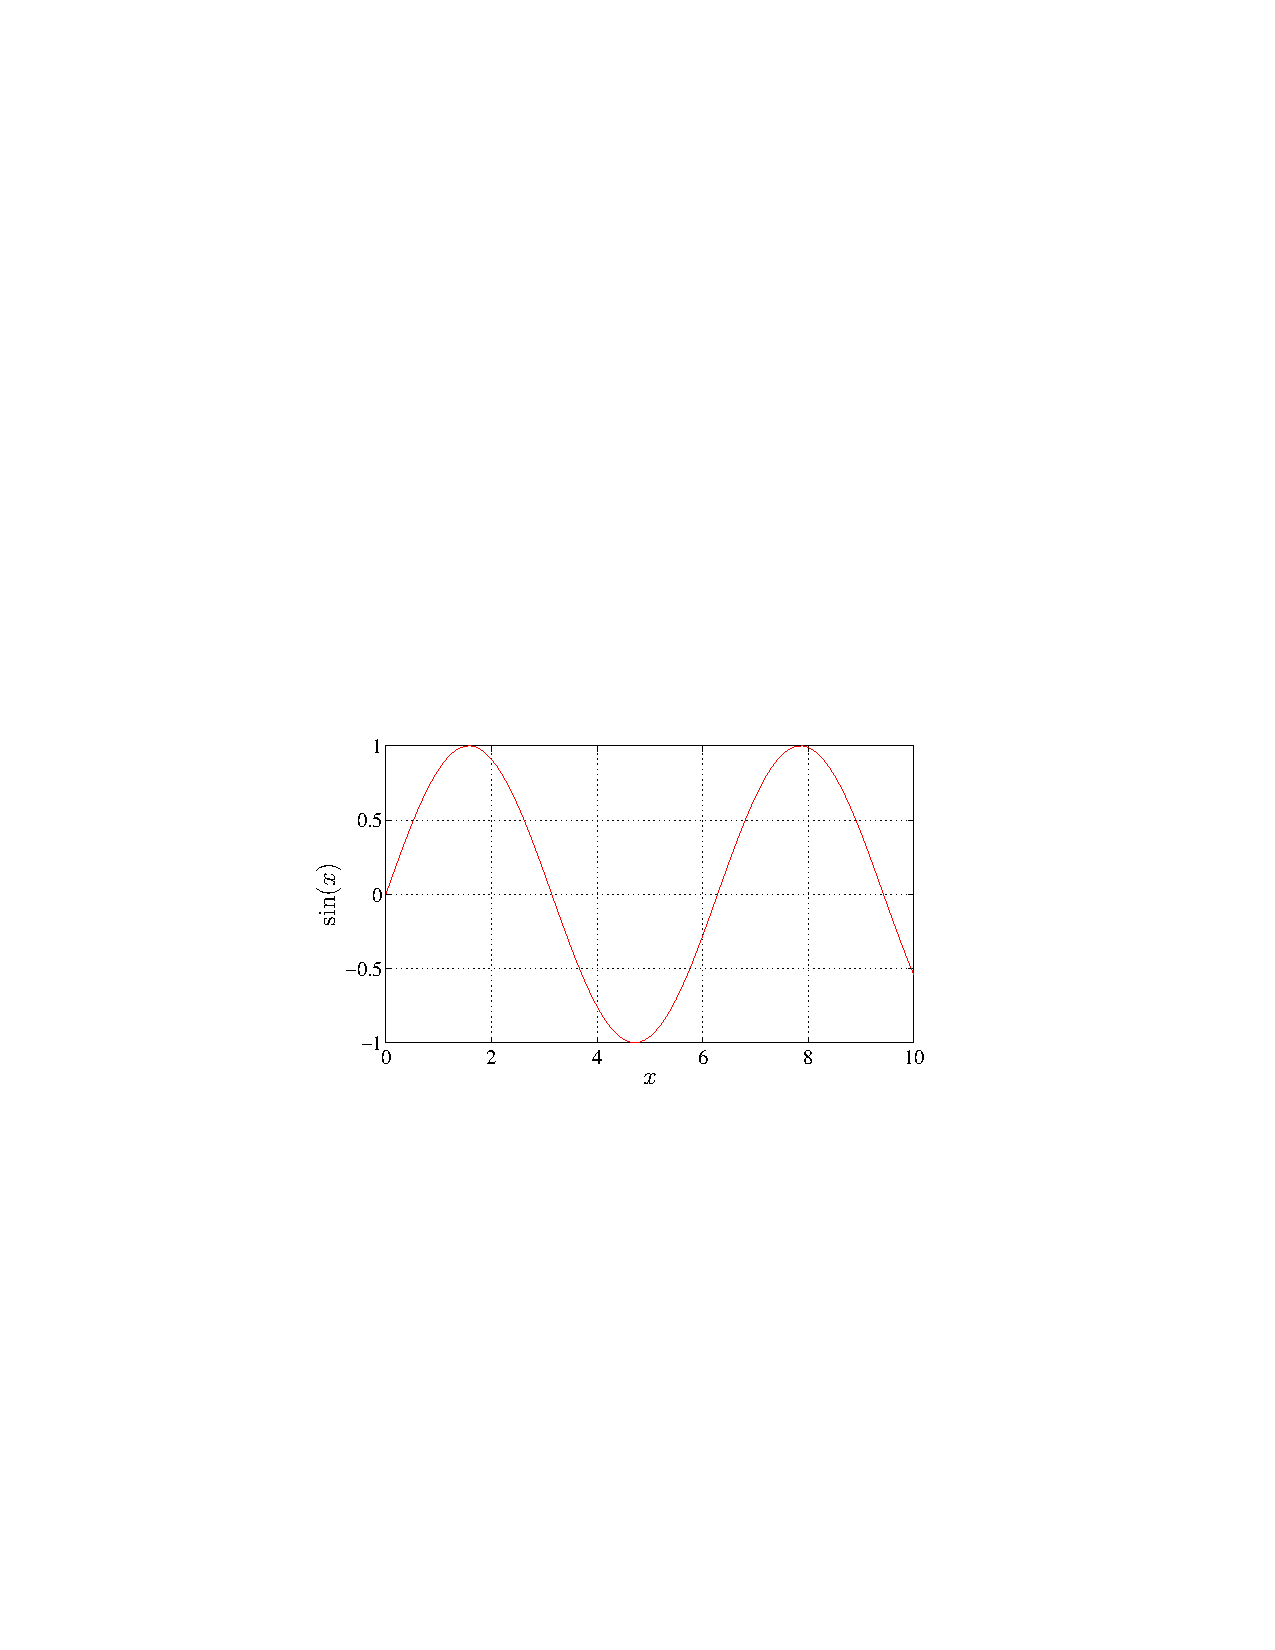
\includegraphics[width=\columnwidth]{fig1a}}
  \caption{Example of a figure with experimental results.}
  \label{fig:results}
\end{figure}

\begin{equation}
  \label{eqn:wave_equation}
    \Delta^2p(x,y,z,t)-
    \displaystyle\frac{1}{c^2}\frac{\partial^2p(x,y,z,t)}{\partial t^2}=0,
\end{equation}



% -------------------------------------------------------------------------
% Either list references using the bibliography style file IEEEtran.bst
\bibliographystyle{IEEEtran}
\bibliography{refs}
%
% or list them by yourself
% \begin{thebibliography}{9}
% 
% \bibitem{dcase2016web}
%   \url{http://www.cs.tut.fi/sgn/arg/dcase2016/}.
%
% \bibitem{IEEEPDFSpec}
%   {PDF} specification for {IEEE} {X}plore$^{\textregistered}$,
%   \url{http://www.ieee.org/portal/cms_docs/pubs/confstandards/pdfs/IEEE-PDF-SpecV401.pdf}.
%
% \bibitem{PDFOpenSourceTools}
%   Creating high resolution {PDF} files for book production with 
%   open source tools, 
%   \url{http://www.grassbook.org/neteler/highres_pdf.html}.
%
% \bibitem{eWilliams1999}
% E. Williams, \emph{Fourier Acoustics: Sound Radiation and Nearfield Acoustic
%   Holography}. London, UK: Academic Press, 1999.
% 
% \bibitem{ieeecopyright}
%   \url{http://www.ieee.org/web/publications/rights/copyrightmain.html}.
%
% \bibitem{cJones2003}
% C. Jones, A. Smith, and E. Roberts, ``A sample paper in conference
%   proceedings,'' in \emph{Proc. IEEE ICASSP}, vol. II, 2003, pp. 803--806.
% 
% \bibitem{aSmith2000}
% A. Smith, C. Jones, and E. Roberts, ``A sample paper in journals,'' 
%   \emph{IEEE Trans. Signal Process.}, vol. 62, pp. 291--294, Jan. 2000.
% 
% \end{thebibliography}


\end{sloppy}
\end{document}
\grid
